\documentclass{beamer}
% \setbeameroption{show notes}
\setbeamertemplate{section in toc}[sections numbered]

\usepackage[spanish,es-ucroman]{babel}
\usepackage[spanish, backgroundcolor=green]{todonotes}
\usepackage[lined,linesnumbered,spanish,onelanguage]{algorithm2e}

\usepackage[beamer,customcolors]{hf-tikz} \hfsetfillcolor{alerted text.fg!10} \hfsetbordercolor{alerted text.fg}

\usetheme[
    language=spanish,
    titlepagelogo=../paper/latex/Graphics/uhlogo,
    pageofpages=de,
    notshowauthor=true,
    secondlogo=true,
    titleline=false,
    color=red
]{TorinoTh}

\setbeamertemplate{headline}{}

\setrellabel{Tutor}
\setcandidatelabel{Tesista} \setassistentsupervisorlabel{Co Tesis} \setsubject{Tesis}

\titlepagesecondlogo{graphics/matcom-logo}
\title{Sistema de Votaci\'on Representativa sobre \textit{Quorum}}
\author{Andy Ledesma Garc\'ia}
\rel{Yaidir Mustelier Ruiz}
\ateneo{Universidad de La Habana. MATCOM}
\date{13 de diciembre de 2022}  % @remind cambiar si la fecha es otro d\'ia

\begin{document}
\titlepageframe

\begin{frame}
    \frametitle{D\'eficit Fiscal}
    \framesubtitle{Monetizaci\'on vs. Endeudamiento P\'ublico}

    \begin{alertblock}{Problema}
        Los ingresos fiscales resultan insuficientes para financiar la actividad del sector público de un país.
    \end{alertblock}

    \pause

    Soluciones:
    \begin{itemize}[<+->]
        \pause

        \item monetizaci\'on de la deuda p\'ublica
        \note[item]<3>{Los bancos financian la deuda p\'ublica}
        \note[item]<3>{Produce inflaci\'on}
        \item endeudamiento p\'ublico
        \note[item]<4>{el estado se endeuda y promete devolver en un tiempo. El monto y cr\'edito de la deuda se plasman en un doc llamado \textbf{bono soberano}}
    \end{itemize}

    \onslide<5->
    \begin{center}
        \Large \highlightbf{Mercado de Deuda P\'ublica}
    \end{center}
\end{frame}

\begin{frame}
    \frametitle{Obtenci\'on del Prestamista}

    \todo[inline]{@TODO pon foto pa ocupar espacio}
    
    \begin{enumerate}
        \pause

        \item $\text{bono soberano} = \text{monto solicitado} + \text{cr\'edito m\'aximo}$
        \item<5-> confecci\'on de los \highlightbf{Comit\'es de Mercado Financiero} 
        \note<5>{
            \begin{itemize}
                \item autoridad de mercado q regirá el reglamento del MDP
                \item adopta las medidas q estime convenientes
                \item tiene potestad disciplinaria sobre todos los operadores del mercado
                \item para su confecci\'on se realiza un proceso de votaci\'on representativa \todo[inline]{@audit c\'omo se determinan espec\'ificamente los candidatos y el presidente?} 
            \end{itemize}
        }
        \item<3-> subasta 
        \note<3>{se subasta a ver ki\'en pide menos cr\'edito}
        \item<4-> prestamista $=$ ganador
    \end{enumerate}
\end{frame}

\begin{frame}
    \frametitle{Sistema de Votaci\'on Representativa}
    \framesubtitle{Definici\'on y Conteo de Votos}

    \includegraphics<1>{../paper/latex/Graphics/rep-voting.pdf}

    \note<1>{
        \begin{itemize}
            \item el poder de voto es transferible, esto implik q un participante puede ser a la vez votante y candidato
            \item a lo sumo un voto por votante
        \end{itemize}
    }
    \includegraphics<2>{graphics/rep-voting-colored-winner.pdf}

    \note<2>[item]{gana $D$}
    \note<2>[item]{en este sistema hay dos problemas principales a enfrentar...}
\end{frame}

\begin{frame}
    \frametitle{Sistema de Votaci\'on Representativa}
    \framesubtitle{Ciclos}

    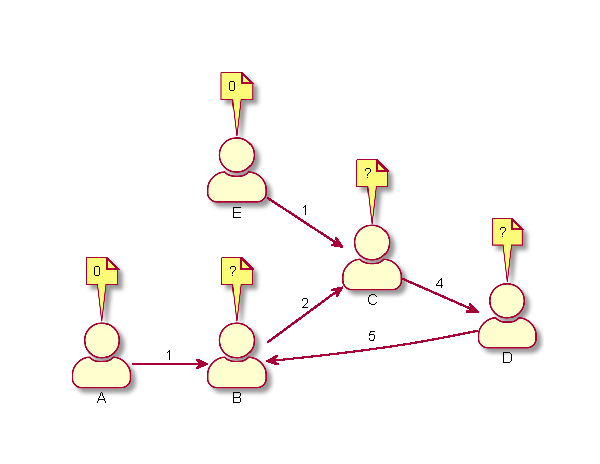
\includegraphics{../paper/latex/Graphics/voting-cycle.pdf}
    \note{no keda claro cu\'antos votos asignar a los del ciclo de manera  justa, de acuerdo con el proceso de votaci\'on}
\end{frame}

\begin{frame}
    \frametitle{Sistema de Votaci\'on Representativa}
    \framesubtitle{Empate en el Primer Lugar}

    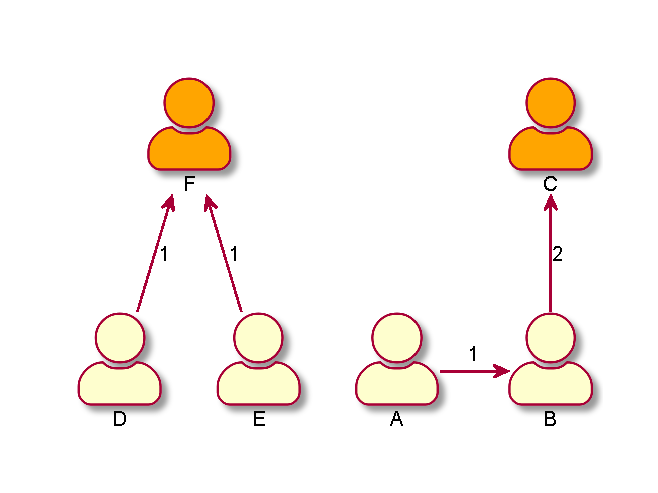
\includegraphics[scale=.9]{graphics/2-winners.pdf}
    \note{
        \begin{enumerate}
            \item hay q seleccionar un solo ganador
            \item s\'olo hay q atender a los empates en el 1er lugar
        \end{enumerate}
    }
\end{frame}

\begin{frame}
    \frametitle{Implementaci\'on en \textit{Quorum}}

    \note<1>{habla a grandes razgos de lo q es Quorum}

    \todo[inline]{@TODO poner logo a la der de quorum}

    \pause

    Por ser un sistema electrónico:
    \begin{adv}
        \item conteo autom\'atico
        \note<2>{Que sea autom\'atico facilita la correctitud y la eficiencia.}
        \item bajos costos 
    \end{adv}

    \pause

    Por ser tecnología \textit{blockchain}:
    \begin{adv}
        \item registro perdurable de votos
        \item sistema descentralizado
    \end{adv}

    \pause

    Ventajas particulares:
    \begin{adv}
        \item el costo  de las transacciones es personalizable
        \item transacciones privadas
        \item contratos inteligentes 
    \end{adv}
\end{frame}

\newcommand{\countsectionname}{contar los votos correctamente}
\newcommand{\cyclecountsectionname}{asignar conteo justo a los candidatos en ciclos}
\newcommand{\onewinneronlysectionname}{obtener s\'olo un ganador}
\newcommand{\quorumimplementationsectionname}{implementar los algoritmos sobre {\it Quorum}}

\begin{frame}
    \frametitle{Objetivos}

    \begin{alertblock}{Objetivo Principal}
        Dise\~nar algoritmos para el desarrollo de sistemas de votaciones representativas sobre \textit{Quorum}.
    \end{alertblock}

    \pause

    Objetivos espec\'ificos:

    \pause

    \begin{enumerate}[<+->]
        \item \countsectionname
        \item \cyclecountsectionname
        \item \onewinneronlysectionname
        \item \quorumimplementationsectionname
    \end{enumerate}
\end{frame}

\note{y ahora vamos a ir respondiendo c\'omo se fueron cumpliendo cada uno de ellos}

\AtBeginSection{
    \begin{frame}<beamer>
        \frametitle{Objetivos Espec\'ificos}
        \tableofcontents[currentsection]
    \end{frame}
}

\section{\countsectionname}
\begin{frame}
    \frametitle{Conteo de Votos}
    \framesubtitle{Definici\'on}

    \begin{center}
        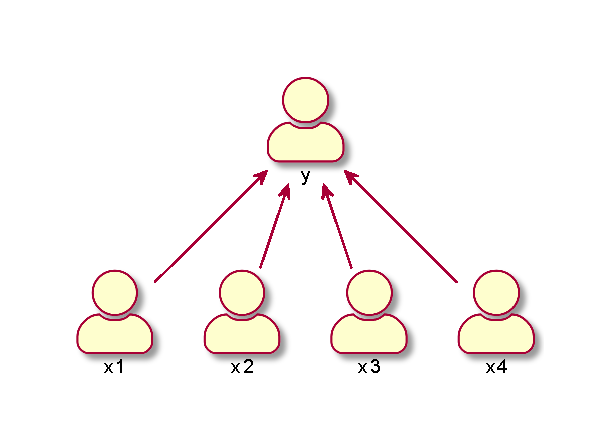
\includegraphics[scale=0.7]{graphics/incoming-votes.pdf}
    \end{center}
    \only<1>{
        $$
        \#_{votos}(y) = \text{\color{red} votos directos} + \text{\color{blue} votos indirectos} 
        $$
    }
    \only<2>{
        $$
        \#_{votos}(y) = \begin{cases}
        {\color{red} |V_y|} + {\color{blue} \underset{x \in V_y}{\sum} \#_{votos}(x)} & \text{si } V_y \neq \emptyset \\
        0 & \text{si } V_y = \emptyset 
        \end{cases}
        $$
    }
\end{frame}

\begin{frame}
    \frametitle{Conteo de Votos}
    \framesubtitle{Invirtiendo Grafo}

    \begin{center}
        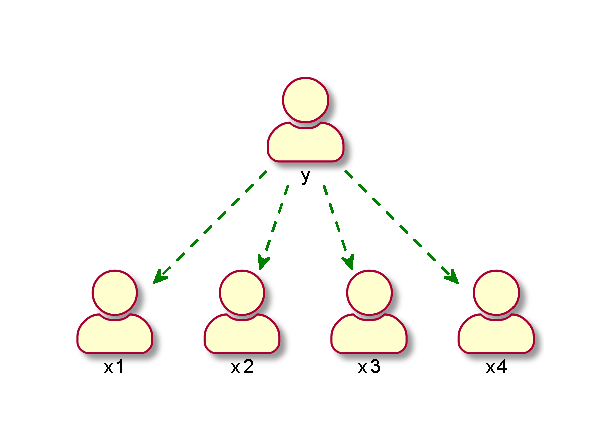
\includegraphics[scale=0.7]{graphics/incoming-votes-inverted-graph.pdf}
    \end{center}
    $$
    \#_{votos}(y) = \begin{cases}
    |V_y| + \underset{x \in V_y}{\sum} \#_{votos}(x) & \text{si } V_y \neq \emptyset \\
    0 & \text{si } V_y = \emptyset 
    \end{cases}
    $$

    \note[item]{en este grafo invertido los arcos representan la dependencia del c\'alculo de $\#_{votos}$}
    \note[item]{dada la naturaleza recursiva de la definici\'on del conteo de votos y la forma del grafo, se hace DFS}
\end{frame}

\begin{frame}
    \frametitle{Conteo de Votos}
    \framesubtitle{Contando con DFS}
    
    \begin{columns}
        \begin{column}{.52\textwidth}
            \begin{center}
                \includegraphics<1>[scale=0.6]{graphics/dfs-all-white.pdf}

                \note<1>{nota q pueden haber v\'ertices q ya sean negros antes de visitar $y$, debido  a llamados previos a DFS-Visit}

                \includegraphics<2-3>[scale=0.6]{graphics/dfs-y-gray.pdf}
                \includegraphics<4>[scale=0.6]{graphics/dfs-x2-gray.pdf}
                \includegraphics<5>[scale=0.6]{graphics/dfs-x2-black.pdf}
                \includegraphics<6>[scale=0.6]{graphics/dfs-x3-gray.pdf}
                \includegraphics<7>[scale=0.6]{graphics/dfs-x3-black.pdf}
                \includegraphics<8>[scale=0.6]{graphics/dfs-x4-gray.pdf}
                \includegraphics<9>[scale=0.6]{graphics/dfs-x4-black.pdf}
                \includegraphics<10>[scale=0.6]{graphics/dfs-y-black.pdf}
            \end{center}
        \end{column}

        \column{.48\textwidth}
        DFS-Visit($y$):
        \begin{algorithm}[H]
            \DontPrintSemicolon

            $\tikzmarkin<2>{a} y.color = \text{GRIS} \tikzmarkend{a}$\; 

            \ForEach{$x \in V_y$}{ 
                \If{$x.color ==$ {\rm BLANCO}}{
                    $\tikzmarkin<4,6,8>{c} \text{DFS-Visit}(x) \tikzmarkend{c} $\;
                }
                \If{$x.color ==$ {\rm NEGRO}}{ 
                    $\tikzmarkin<3,5,7,9>{b} y.votos += 1 + x.votos \tikzmarkend{b} $\; 
                }
            }
            $\tikzmarkin<10>{d} y.color = \text{NEGRO} \tikzmarkend{d}$\;
        \end{algorithm}
    \end{columns}
\end{frame}

\section{\cyclecountsectionname}

\begin{frame}
    \frametitle{Candidatos en Ciclo}
    \framesubtitle{M\'aximo N\'umero de Votos}

    \begin{center}
        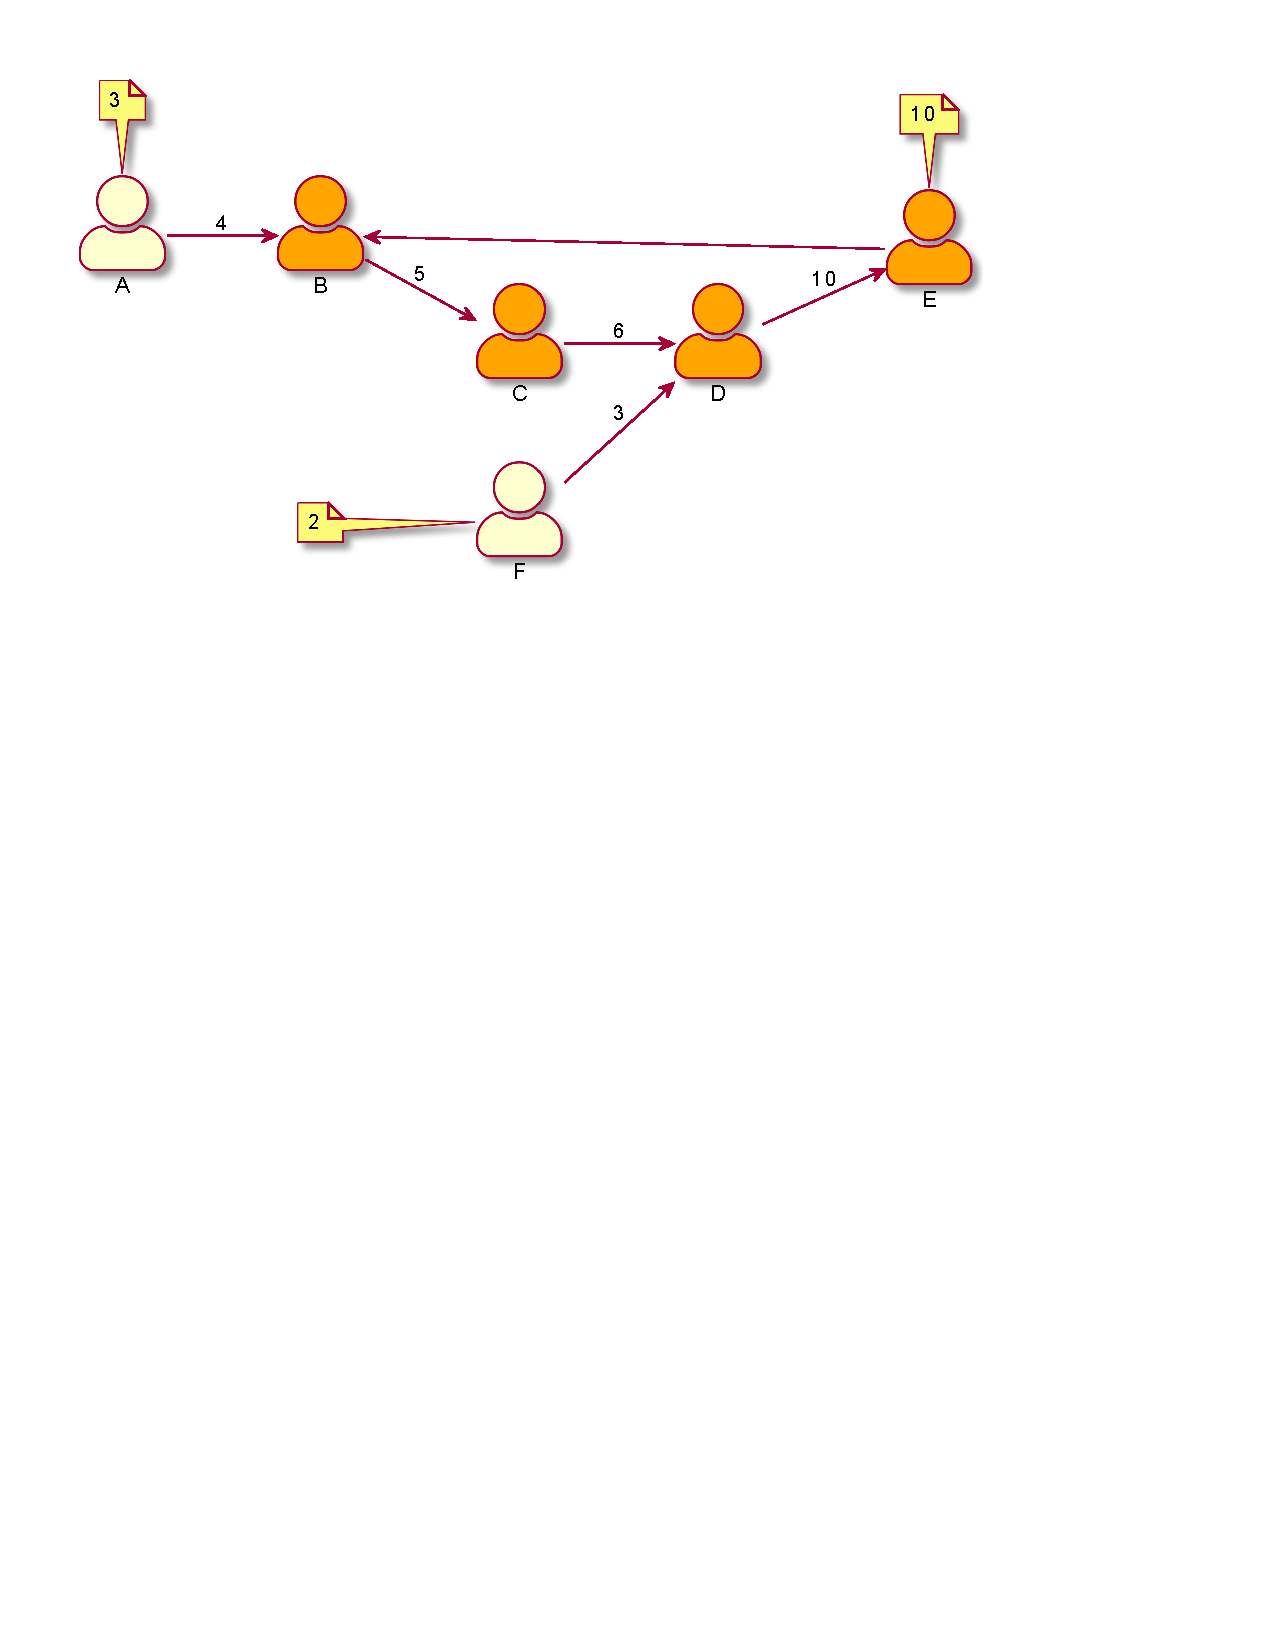
\includegraphics[scale=0.65]{graphics/max-votes-in-cycle.pdf}
    \end{center}

\end{frame}

\begin{frame}
    \frametitle{Candidatos en Ciclo}
    \framesubtitle{Reasignando Votos}

    \begin{center}
        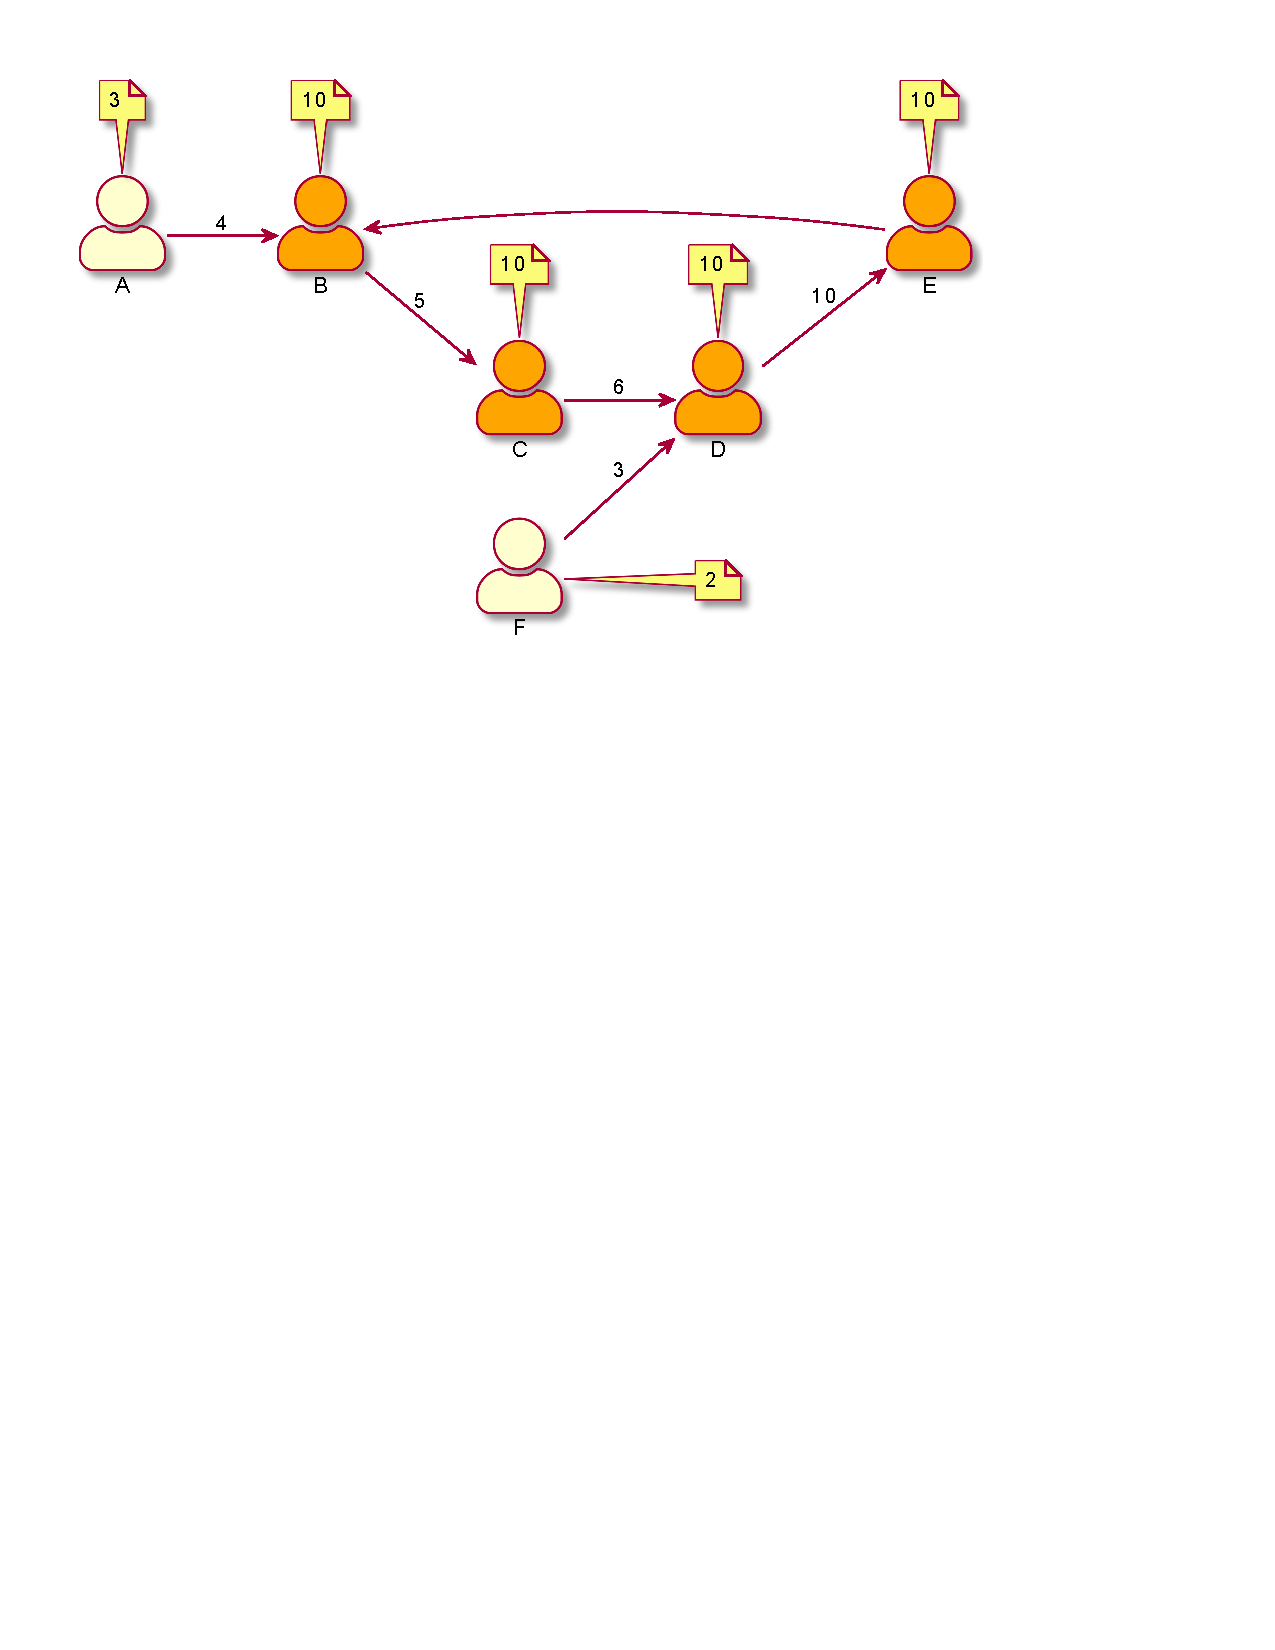
\includegraphics[scale=0.6]{graphics/same-votes-in-cycle.pdf}
    \end{center}

    \note[item]{se detectan los ciclos en el algoritmo DFS-Visit cuan2 se encuentra un arco entre v\'ertices grises}
    \note[item]{luego q todo el DFS termina, es q se reasignan los votos}
\end{frame}

\section{\onewinneronlysectionname}

\begin{frame}
    \frametitle{habla mi'o}

    

\end{frame}

\section{\quorumimplementationsectionname}

\begin{frame}
    \frametitle{habla mi'o}

\end{frame}

\end{document}